\documentclass[11pt,a4paper]{article}
\usepackage[T1]{fontenc}
\usepackage[utf8]{inputenc}
\usepackage[margin=2.15cm]{geometry}
\usepackage{setspace}
\setstretch{1.08}
\usepackage{amsmath,amssymb}
\usepackage{graphicx}
\usepackage{booktabs}
\usepackage{tikz}
\usetikzlibrary{arrows.meta,positioning}
\usepackage[hidelinks]{hyperref}
\newcommand{\vect}[1]{\mathbf{#1}}
\graphicspath{{../paper/figs/}}
\setlength{\parskip}{0.35em}
\setlength{\parindent}{1.15em}

\title{\textbf{A Vibration--Wavelet--Coefficient Feature\\ for Rotating-Machinery Faults}}
\author{Short paper on the first innovation of the expanded study\\
based on You, Fan, Li, Liang, Fang, and Wang,\\
\textit{Shock and Vibration}, 2019, Article ID 1908485}
\date{}

\begin{document}
\maketitle
\thispagestyle{empty}
\vspace{-1.6em}

\begin{abstract}
\noindent
Fault description for a vertical axial-flow pump has to keep three facts that a single transform discards.
Vibration severity measures how hard the casing is moving, and on this rig it separates an eccentric axle from healthy running while leaving a bearing-pedestal fault almost unchanged.
A dyadic wavelet energy time-spectrum shows which scale carries the record, so a short transient is not averaged away by one Fourier transform of the whole capture.
The coefficient power spectrum of that loudest scale then reads seven shaft orders, from half order through the sixth harmonic, on the radial, tangential, and axial channels.
One severity scalar and twenty-one spectral samples form the vibration--wavelet--coefficient (VWC) vector in $\mathbb{R}^{22}$.
This short paper specifies that map, shows why the three blocks are not substitutes for one another, and records what the published pump signatures look like inside it.
The vector is the common input of every classifier in the parent study.
The search that labels it is a separate innovation.
\end{abstract}

\section{Introduction}

A rotating machine writes its condition into casing acceleration, but the raw record is the wrong object to classify.
At the duty used here the shaft turns at $960\,\mathrm{r/min}$, so the fundamental is $f_0=n/60=16\,\mathrm{Hz}$, and a capture of $8192$ samples at $10\,\mathrm{kHz}$ lasts $0.8192\,\mathrm{s}$, about $13.1$ revolutions, with a Fourier bin of $1.221\,\mathrm{Hz}$.
That grid resolves $3f_0=48\,\mathrm{Hz}$ from the $50\,\mathrm{Hz}$ supply line.
It does not by itself say which number a maintenance decision needs.

Three descriptions compete.
Root-mean-square velocity, the vibration severity, is the standardized intensity \cite{iso20816}.
On the published radial records it is $1.051\,\mathrm{mm/s}$ when the pump is healthy, $3.737\,\mathrm{mm/s}$ with an eccentric axle, $1.161\,\mathrm{mm/s}$ with a bearing-pedestal fault, and $1.700\,\mathrm{mm/s}$ with sealing-ring wear \cite{you2019}.
The eccentric state is obvious on this axis.
The pedestal state is a ten-percent change and cannot be thresholded safely.
A single Fourier spectrum of the whole capture sees shaft orders and also averages any impact that does not last for the $0.82\,\mathrm{s}$ record \cite{peng2004}.
A wavelet energy vector sees the loud scale and does not say whether the loudness sits at $8\,\mathrm{Hz}$ or at $16\,\mathrm{Hz}$ \cite{mallat1989}.
VWC keeps all three, and nothing else, so the interface to a classifier stays a vector of dimension $22$.

The mechanical vocabulary is fixed by the shaft.
The orders sampled from the loudest scale are
\begin{equation}
\mathcal{F}=\bigl\{\tfrac12 f_0,\,f_0,\,2f_0,\,3f_0,\,4f_0,\,5f_0,\,6f_0\bigr\}
=\{8,16,32,48,64,80,96\}\,\mathrm{Hz}.
\label{eq:F}
\end{equation}
Half order is the signature of a motion that repeats every two revolutions, as a loose pedestal can.
The first order is the unbalance line.
The fourth order is also blade pass, because the impeller has four blades: $4\times 16=64\,\mathrm{Hz}$.
A line at $64\,\mathrm{Hz}$ is therefore expected in the healthy machine.

\section{The three blocks}

\subsection{Severity}

If $v(t)$ is vibration velocity over a record of length $T$, severity is the RMS velocity
\begin{equation}
\mathrm{VIB}=\sqrt{\frac{1}{T}\int_0^{T} v(t)^2\,\mathrm{d}t}
=\sqrt{\frac{1}{n}\sum_{i=0}^{n-1} v_i^2}.
\label{eq:vib}
\end{equation}
The parent study's source accumulates absolute acceleration over a $10\,\mathrm{ms}$ window to obtain the velocity series that enters \eqref{eq:vib} \cite{you2019}.
That window is about one sixth of a revolution at $16\,\mathrm{Hz}$, and the absolute value makes the sample a local intensity rather than a signed integral.
The published millimetre-per-second figures are used under that definition.
Figure~\ref{fig:sev} restates them.
Severity contributes one coordinate, the radial value, because seven orders on three axes already give $21$ numbers and the full vector has length $22$.

\begin{figure}[ht]
\centering
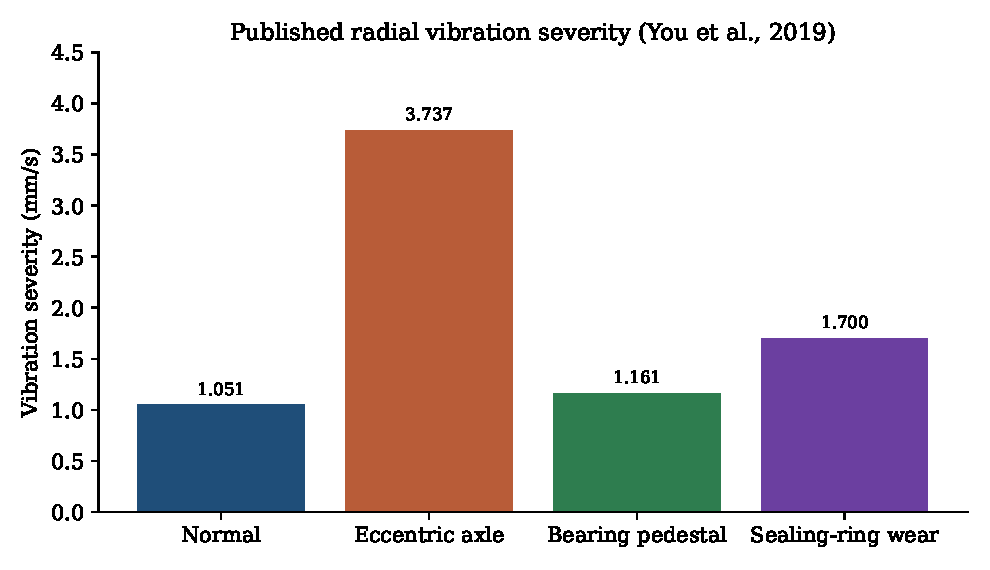
\includegraphics[width=0.72\textwidth]{severity.pdf}
\caption{Published radial vibration severity. Eccentricity multiplies the healthy value by about $3.56$. The pedestal fault multiplies it by about $1.10$.}
\label{fig:sev}
\end{figure}

\subsection{Dyadic energy}

A mother wavelet $\psi$ of zero mean and unit norm generates the dyadic family $\psi_{2^j,b}(t)=2^{-j/2}\psi(2^{-j}(t-b))$.
On a sampled record the inner products are the detail coefficients of Mallat's filter bank \cite{mallat1989,daubechies1988}.
One analysis step convolves the current approximation with a low-pass filter $h$ and a high-pass filter $g$, then downsamples both branches by two.
The high-pass branch at level $j$ is $cD^{j}$.
The energy time-spectrum at that scale is the squared coefficient sequence
\begin{equation}
E(2^{j})[k]=\lvert cD^{j}[k]\rvert^{2},
\label{eq:E}
\end{equation}
and the scalar that ranks scales is the sum $\mathcal{E}(2^{j})=\sum_k E(2^{j})[k]$.
The winning index $k^{\star}$ is any level of maximum $\mathcal{E}$, with a tie broken toward the finer level so that a transient is preferred to a trend of equal energy.
The map does not hard-code level $5$.
The source plots happen to show $d_5$ as the loudest detail, which is consistent with acceleration energy sitting in a structural band near a few hundred hertz while the shaft family itself is coarser.
With $f_s=10\,\mathrm{kHz}$, ideal half-bands put $d_5$ near $156$--$312\,\mathrm{Hz}$.
The shaft orders are still readable at that level because they modulate the resonant carrier, and because the coefficient rate $f_s/2^{5}=312.5\,\mathrm{Hz}$ has Nyquist frequency $156.25\,\mathrm{Hz}$, above $6f_0=96\,\mathrm{Hz}$.

\subsection{Coefficient power spectrum}

The third block is the power spectrum of the energy time series at the winning level,
\begin{equation}
E_{p}(\omega,2^{k^{\star}})
=\frac{1}{N_c}\left\lvert\sum_{n=0}^{N_c-1} E(2^{k^{\star}})[n]\,e^{-i\omega n/N_c}\right\rvert^{2},
\label{eq:cps}
\end{equation}
with coefficient-domain frequency mapped back to hertz by $f=\nu\cdot f_s/2^{k^{\star}}$.
Each feature is the sample of \eqref{eq:cps} nearest an order in $\mathcal{F}$, taking the strongest bin inside half a shaft order if the line falls between bins.
That window is $4\,\mathrm{Hz}$ at this speed, narrower than the $2\,\mathrm{Hz}$ gap from $48\,\mathrm{Hz}$ to the supply, so the sampler does not report mains as $3f_0$.
An order above the coefficient Nyquist of $k^{\star}$ is refused rather than folded.

\section{The vector, and what the four states do in it}

Concatenate the radial severity with the seven amplitudes on each axis:
\begin{equation}
\begin{aligned}
\vect{x}=\bigl(&\mathrm{VIB}_{r},\;
p_{t}(\eta),\; p_{a}(\eta),\; p_{r}(\eta)
\bigr)^{\top},
\qquad \eta\in\mathcal{F}.
\end{aligned}
\label{eq:x}
\end{equation}
Training and test rows must use the same coordinate order.
Before classification, each coordinate is scaled to the unit interval by a range fit on the training rows only and frozen for the test rows.
Severity is near $1\,\mathrm{mm/s}$ and a coefficient power sample is near $10^{-3}$; without this map the radial kernel would ignore the spectral block.

The published reading of the pump records is then a statement about $\vect{x}$ \cite{you2019}.
Healthy running pairs a moderate severity with a tangential spectrum peaked at $16\,\mathrm{Hz}$.
The published tangential peak power there is $1.683\times 10^{-3}$.
Eccentric axle raises severity by the factor $3.56$ and raises that tangential peak to $3.322\times 10^{-3}$, which is the stationary form of a larger unbalance force.
Bearing-pedestal fault leaves severity almost alone and moves the tangential peak to $8\,\mathrm{Hz}$, at a published power $4.701\times 10^{-3}$, about $2.8$ times the healthy tangential peak.
Sealing-ring wear sets severity at $1.70\,\mathrm{mm/s}$ and emphasizes $f_0$, half order, and $2f_0$, with the tangential channel again the largest.
The pedestal ratio is the empirical reason the vector contains both blocks: the spectral coordinate moves by a larger factor than the severity coordinate.
Figure~\ref{fig:spec} is an illustrative baseband picture of that emphasis, not a laboratory spectrum.

\begin{figure}[ht]
\centering
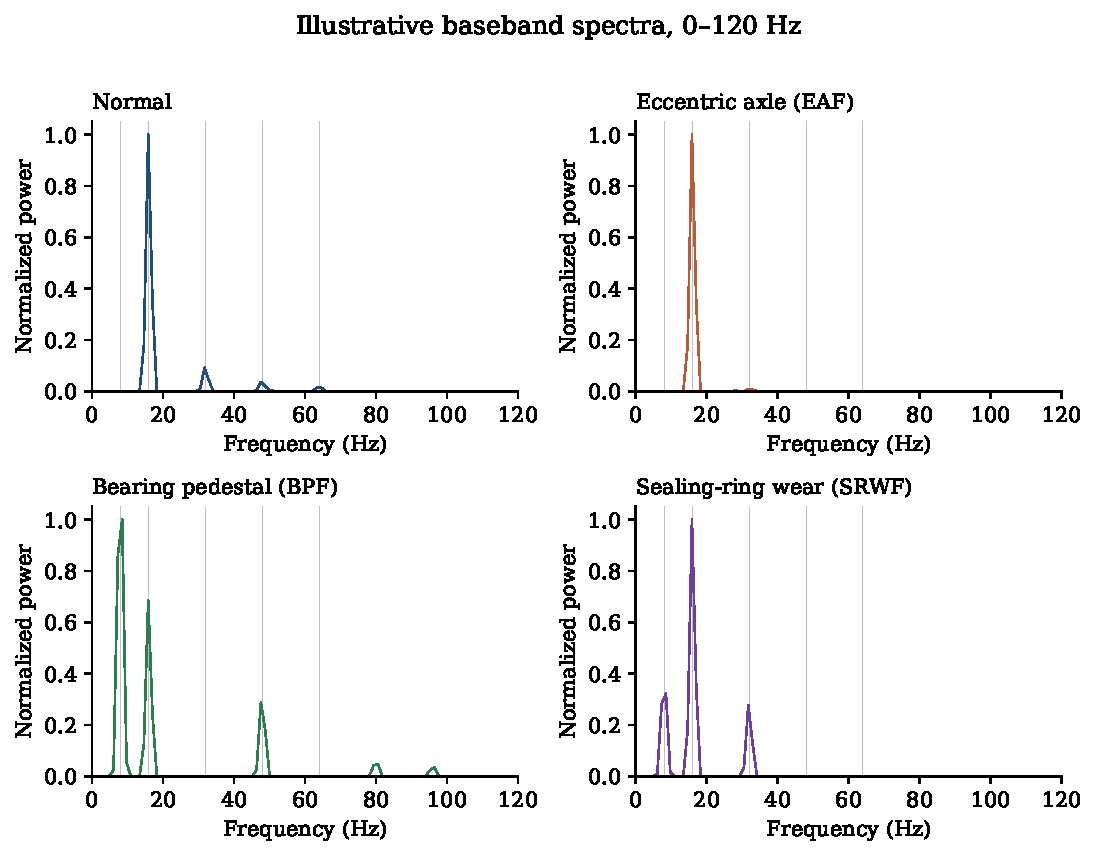
\includegraphics[width=0.92\textwidth]{spectra.pdf}
\caption{Illustrative baseband spectra shaped to the published emphasis. They are not the laboratory recordings.}
\label{fig:spec}
\end{figure}

\begin{figure}[ht]
\centering
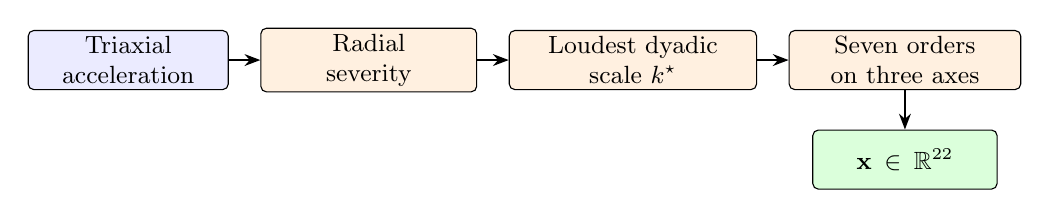
\begin{tikzpicture}[
  box/.style={draw, rounded corners=2pt, align=center, font=\small, inner sep=2pt, minimum height=7.5mm},
  arr/.style={-{Stealth[length=2mm]}, thick}]
\node[box, fill=blue!8, text width=24mm] (a) {Triaxial\\acceleration};
\node[box, fill=orange!12, text width=26mm, right=4mm of a] (v) {Radial\\severity};
\node[box, fill=orange!12, text width=30mm, right=4mm of v] (w) {Loudest dyadic\\scale $k^{\star}$};
\node[box, fill=orange!12, text width=28mm, right=4mm of w] (c) {Seven orders\\on three axes};
\node[box, fill=green!14, text width=22mm, below=5mm of c] (x) {$\vect{x}\in\mathbb{R}^{22}$};
\draw[arr] (a)--(v); \draw[arr] (v)--(w); \draw[arr] (w)--(c); \draw[arr] (c)--(x);
\end{tikzpicture}
\caption{VWC is a concatenation. The classifier never sees the raw record.}
\label{fig:flow}
\end{figure}

\section{What this innovation does and does not do}

VWC is deterministic once the wavelet, the depth, the integrator, and the tie break are fixed.
This specification uses the Daubechies wavelet with four vanishing moments and eight levels, which the 2019 paper does not name; the name is part of the exposition, and the definition of $k^{\star}$ does not depend on it.
The map costs one linear filter bank per axis plus one Fourier transform of the winning coefficient sequence.
At $N=8192$ that cost is negligible beside any later parameter search.
Two hundred and forty vectors, sixty per state, are the entire labeled sample the vector is asked to support \cite{you2019}.

The innovation does not label the vector.
Healthy, eccentric, pedestal, and seal-wear patterns still overlap, and the pedestal pattern is the least stable because resonance and site interference occupy the same high orders the fault uses.
Every classifier that later reads $\vect{x}$ misses at least two of the fifteen pedestal test vectors.
That residue is a property of the measurement, and a different feature map would have to be estimated on a new split before it could be claimed as a repair.
Severity alone is already known to be insufficient: a threshold between $2$ and $3\,\mathrm{mm/s}$ catches the eccentric axle and misses the other two faults.
The $22$-vector is the object that makes the half-order pedestal move and the seal-wear second harmonic available to a margin classifier at the same time as the standardized intensity.

\section{Conclusion}

The first innovation replaces an unstructured vibration record with a $22$-dimensional description: radial vibration severity, the identity of the loudest dyadic scale, and the coefficient power of seven shaft orders on three casing axes.
The blocks answer different questions, and the published severities show that the intensity question and the order question disagree on the pedestal fault.
The map is specified completely enough to implement, including the training-only scale and the refusal of an order that the winning scale cannot represent.
Labels for the vector are the subject of the companion short paper on the modified frog-leaping search.

\begin{thebibliography}{9}
\bibitem{you2019}
L.~You, W.~Fan, Z.~Li, Y.~Liang, M.~Fang, and J.~Wang,
``A fault diagnosis model for rotating machinery using VWC and MSFLA-SVM based on vibration signal analysis,''
\textit{Shock and Vibration}, vol.~2019, Article ID 1908485, 2019.
\bibitem{mallat1989}
S.~G.~Mallat,
``A theory for multiresolution signal decomposition: the wavelet representation,''
\textit{IEEE Trans.\ Pattern Analysis and Machine Intelligence}, vol.~11, no.~7, pp.~674--693, 1989.
\bibitem{daubechies1988}
I.~Daubechies,
``Orthonormal bases of compactly supported wavelets,''
\textit{Comm.\ Pure Appl.\ Math.}, vol.~41, no.~7, pp.~909--996, 1988.
\bibitem{peng2004}
Z.~K.~Peng and F.~L.~Chu,
``Application of the wavelet transform in machine condition monitoring and fault diagnostics: a review,''
\textit{Mechanical Systems and Signal Processing}, vol.~18, no.~2, pp.~199--221, 2004.
\bibitem{iso20816}
International Organization for Standardization,
\textit{ISO 20816-1:2016, Mechanical vibration --- Measurement and evaluation of machine vibration --- Part 1}.
Geneva, 2016.
\bibitem{randall2011}
R.~B.~Randall and J.~Antoni,
``Rolling element bearing diagnostics---a tutorial,''
\textit{Mechanical Systems and Signal Processing}, vol.~25, no.~2, pp.~485--520, 2011.
\end{thebibliography}

\end{document}
